\chapter{Arhitectura}

\paragraph{}
Modelarea unui limbaj reprezint\u a o sarcin\u a extrem de dificil\u a pentru un calculator. Recente progrese \^ in aria Deep Learning au f\u acut posibile diverse dezvolt\u ari \^ in aceast\u a direc\c tie, \^ ins\u a lucrurile sunt departe de a fi rezolvate. Arhitectura folosit\u a pentru construc\c tia chatbot-ului prezentat \^ in aceast\u a lucrare va fi expus\u a precum un bloc de construc\c tii, plec\^ and de la no\c tiunile de baz\u a, p\^ an\u a la arhitectura final\u a.

\section{Re\c tele neurale artificiale}

\paragraph{}
O re\c tea neural\u a artificial\u a (RNA) reprezint\u a o paradigm\u a bazat\u a pe procesare de informa\c tii a c\u arei inspira\c tii provine din sistemul nervos biologic. Precum creierul uman, o RNA este compus\u a dintr-un num\u ar mare de elemente de procesare interconectate (neuroni) lucr\^ and la unison pentru a rezolva diverse probleme. RNA, precum oamenii, \^ inva\c t\u a din exemple. \^ Inv\u a\c tarea \^ in sistemele biologice implic\u a ajustarea conexiunilor sinaptice care exist\u a \^ intre neuroni. Acest principiu se aplic\u a \c si acestor re\c tele.

\paragraph{}
Ca \c si modelare matematic\u a propriu-zis\u a, o RNA poate fi observat\u a \^ in Figura 3.1. Avem o intrare reprezentat\u a \^ in figur\u a de vectorul n-dimensional (x1, x2, x3, x4). Aceast\u a intrare reprezint\u a caracteristicile unui e\c santion care face parte dintr-un set de date. Straturile intermediare se numesc straturi ascunse, iar rolul lor este s\u a produc\u a o abstractizare c\^ at mai complex\u a a datelor de intrare, folosind diverse func\c tii cu activare neliniar\u a. Ultimul strat se nume\c ste strat de ie\c sire, reprezent\^ and eticheta (clasa) vectorului de intrare.

\begin{figure}[H]
\centering
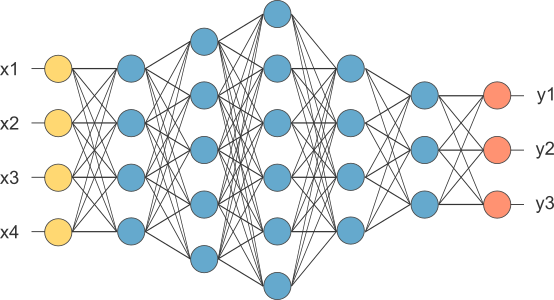
\includegraphics[width=0.7\textwidth]{deep_neural_network}
\caption{Exemplu de re\c tea neural\u a artificial\u a}
\end{figure}

\paragraph{}
Ceea ce de fapt acest tip de re\c tele incearc\u a s\u a inve\c te sunt ponderile dintre straturile sale. Se pleac\u a de la un set de ponderi alese aleator \footnote{Valorile ponderilor sunt deobicei subunitare iar ini\c tializarea este f\u acut\u a urm\^ and diverse principii matematice bine definite. Pentru cazuri simpliste, ini\c tializarea poate fi totu\c si facut\u a folosind o distribu\c tie uniform\u a.} \c si se ajusteaz\u a folosind algoritmul de propagare \^ inapoi a erorii p\^ an\u a c\^and re\c teaua se stabilizeaz\u a. 

\section{Re\c tele neurale artificiale recurente}

\paragraph{}
Dup\u a cum se poate observa, o RNA este util\u a atunci c\^ and intrarea este format\u a dintr-un singur element, de exemplu o imagine. Modelarea unui limbaj \^ ins\u a presupune ca intr\u arile s\u a fie fraze. O fraz\u a este format\u a din mai multe elemente (cuvinte), deci o RNA nu poate modela o astfel de intrare. Solu\c tia pentru aceast\u a problem\u a este oferit\u a de re\c telele neurale artificiale recurente (RNAR). Acestea sunt folosite pentru a modela secven\c te unde exist\u a o dependen\c t\u a temporal\u a (fraze, serii de timp). Fiecare intrare curent\u a din secven\c t\u a este condi\c tionat\u a de cele precedente. O astfel de re\c tea se poate observa \^ in Figura 3.2. Straturile ascunse \^ intr-o RNAR au rolul de a p\u astra o captur\u a a tot ceea ce s-a oferit ca intrare p\^ an\u a \^ in momentul curent. Valoarea fiec\u arui strat ascuns curent depinde astfel at\^ at de intrarea curent\u a c\^ at \c si de ie\c sirea stratului ascuns anterior. Putem considera toat\u a aceast\u a modelare ca pe o probabilitate condi\c tionat\u a \( P(x_{n} | x_{1}, x_{2},..., x_{n-1}) \), unde \^ in cazul unei fraze \(x_{1}, x_{2},..., x_{n}\) reprezint\u a cuvintele acesteia. 

\begin{figure}[H]
\centering
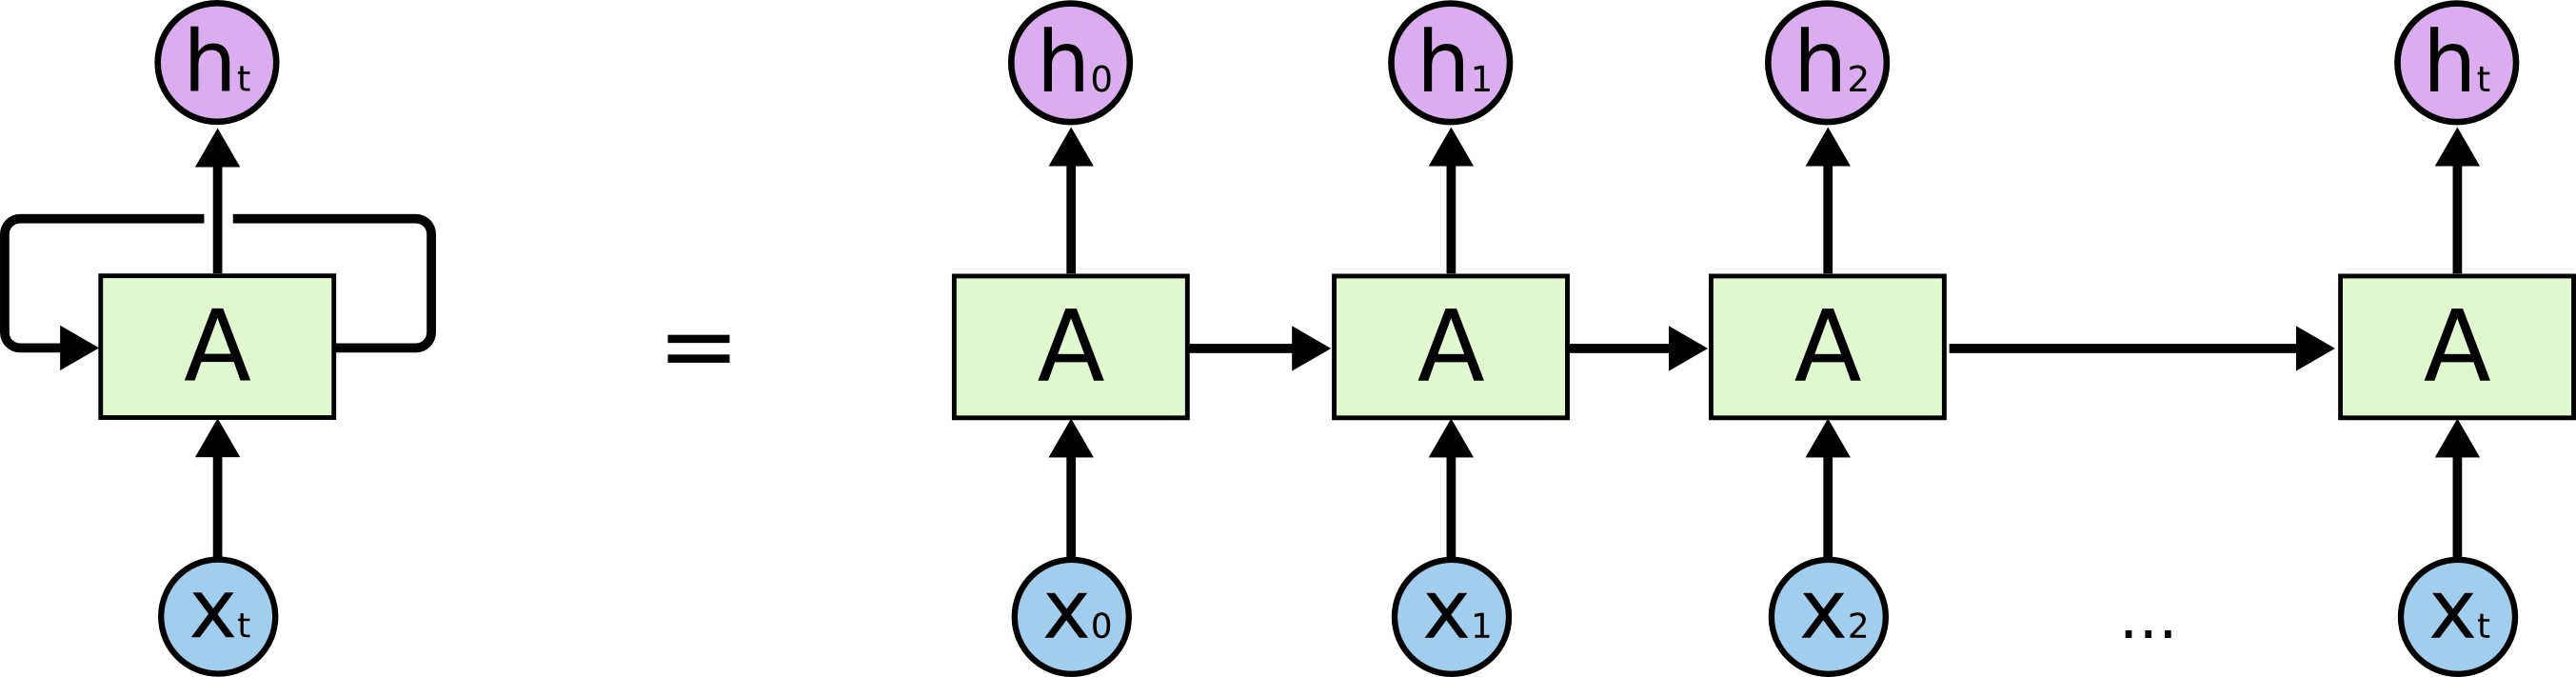
\includegraphics[width=0.9\textwidth]{rnn_network}
\caption{Exemplu de re\c tea neural\u a artificial\u a recurent\u a}
\end{figure}

\paragraph{}
Algoritmul de reglare a ponderilor se nume\c ste propagarea \^ inapoi \^ in timp a erorii. O problem\u a serioas\u a care a ap\u arut odat\u a cu introducerea acestor re\c tele se nume\c ste risipirea gradien\c tilor. \^ In cazul \^ in care secven\c ta de intrare are o lungime mare, informa\c tia nu reu\c se\c ste s\u a se propage \^ in timp deoarece gradientul ponderilor se risipe\c ste, ponderile devenind 0. Mecanismul care \^ inl\u atur\u a aceast\u a problem\u a se nume\c ste Long Short Term Memory (LSTM). Principiul este ca prin folosirea unor por\c ti de transmitere a informa\c tiei, gradientul s\u a fie stabilizat. Acest mecanism a reprezentat un avans spectaculos pentru Deep Learning, permi\c t\^ and modelarea secven\c tial\u a cu re\c tinere a informa\c tiei pe o perioad\u a \^ indelungat\u a de timp. Ecua\c tiile 3.1 descriu calculele pentru por\c tile LSTM.

\begin{equation}
\begin{split}
f_{t} = \sigma(W_{f}x_{t} + U_{f}h_{t-1} + b_{f})\\
i_{t} = \sigma(W_{i}x_{t} + U_{i}h_{t-1} + b_{i})\\
o_{t} = \sigma(W_{o}x_{t} + U_{o}h_{t-1} + b_{o})\\
c_{t} = f_{t} \circ c_{t-1} + i_{t} \circ \tanh (W_{c}x_{t} + U_{c}h_{t-1} + b_{c})\\
h_{t} = o_{t} \circ \tanh (c_{t})\\
\end{split}
\end{equation}

\paragraph{}
Poarta \(f_{t}\) se nume\c ste poart\u a de uitare (forget gate). Rolul ei este s\u a stabilieasc\u a c\^ at\u a informa\c tie se va uita din trecut. Poarta \(i_{t}\) este poarta de intrare (input gate). Aceasta delimiteaz\u a care este cantitatea de informa\c tie care se p\u astreaz\u a din intrarea curent\u a. Poarta \(o_{t}\) este cea de ie\c sire (output gate). Ea controleaz\u a ce informa\c tie va fi transmis\u a c\u atre ie\c sire. \(c_{t}\) se nume\c ste starea intern\u a a celulei LSTM. Aceasta este calculat\u a ca o combina\c tie \^ intre starea anterioar\u a a celulei, poarta de intrare \c si cea de ie\c sire. \(h_{t}\) reprezint\u a ie\c sirea curent\u a a re\c telei \c si depinde de poarta de ie\c sire \c si starea celulei LSTM. 

\paragraph{}
O RNAN aduce mai aproape ideea de modelare lingvistica, \^ ins\u a se poate observa c\u a aceasta nu permite ca intrare dec\^ at o fraz\u a pe r\^ and. Modelarea dorit\u a este o pereche de forma \^ intrebare-r\u aspuns.

\section{Modele Sequence-to_Sequence}

